% !TEX root = ../thesis.tex

\vspace{-20pt}

\section{Interactive Selections}
\label{sec:vl:goi}

\vspace{-10pt}

To support specification of interaction techniques, we extend the definition of
unit specifications to also include a set of \emph{selections}. Selections
identify the set of points a user is interested in manipulating, and is formally
defined as an eight-tuple:

\vspace{7pt}
\centerline{
  \emph{selection := (name, type, predicate, domain$|$range, event, init,
  transforms, resolve})
}

When an input \emph{event} occurs, the selection is populated with \emph{backing
points} of interest. These points are the minimal set needed to identify all
\emph{selected points}. The selection \emph{type} determines how many backing
values are stored, and how the \emph{predicate} function uses them to determine
the set of selected points. Supported types include a \emph{single} point,
\emph{multiple} discrete points, or a continuous \emph{interval} of points.

As its name suggests, a single selection is backed by one datum, and its
predicate tests for an exact match against properties of this datum. It can also
function like a dynamic variable (or \emph{signal} in
Vega~\cite{reactive-vega-model}), and can be invoked as such. For example, it
can be referenced by name within a filter expression, or its values used
directly for particular encoding channels. \emph{Multi} selections, on the other
hand, are backed by datasets into which data values are inserted, modified or
removed as events fire. They express discrete selections, as their predicates
test for an exact match with at least one value in the backing dataset. The
order of points in a multi selection can be semantically meaningful, for example
when a multi selection serves as an ordinal scale domain.
\Cref{fig:vl:singleSelection,fig:vl:multiSelection} illustrate how points are
highlighted in a scatterplot using single and multi selections.

Intervals are similar to multi selections. They are backed by datasets, but
their predicates determine whether an argument falls within the minimum and
maximum extent defined by the backing points. Thus, they express continuous
selections. The compiler automatically adds a rectangle mark, as shown in
\cref{fig:vl:intervalSelection}, to depict the selected interval. Users can
customize the appearance of this mark via the \texttt{mark} keyword, or disable
it altogether when defining the selection.

\begin{figure*}[h!]
  \centering
  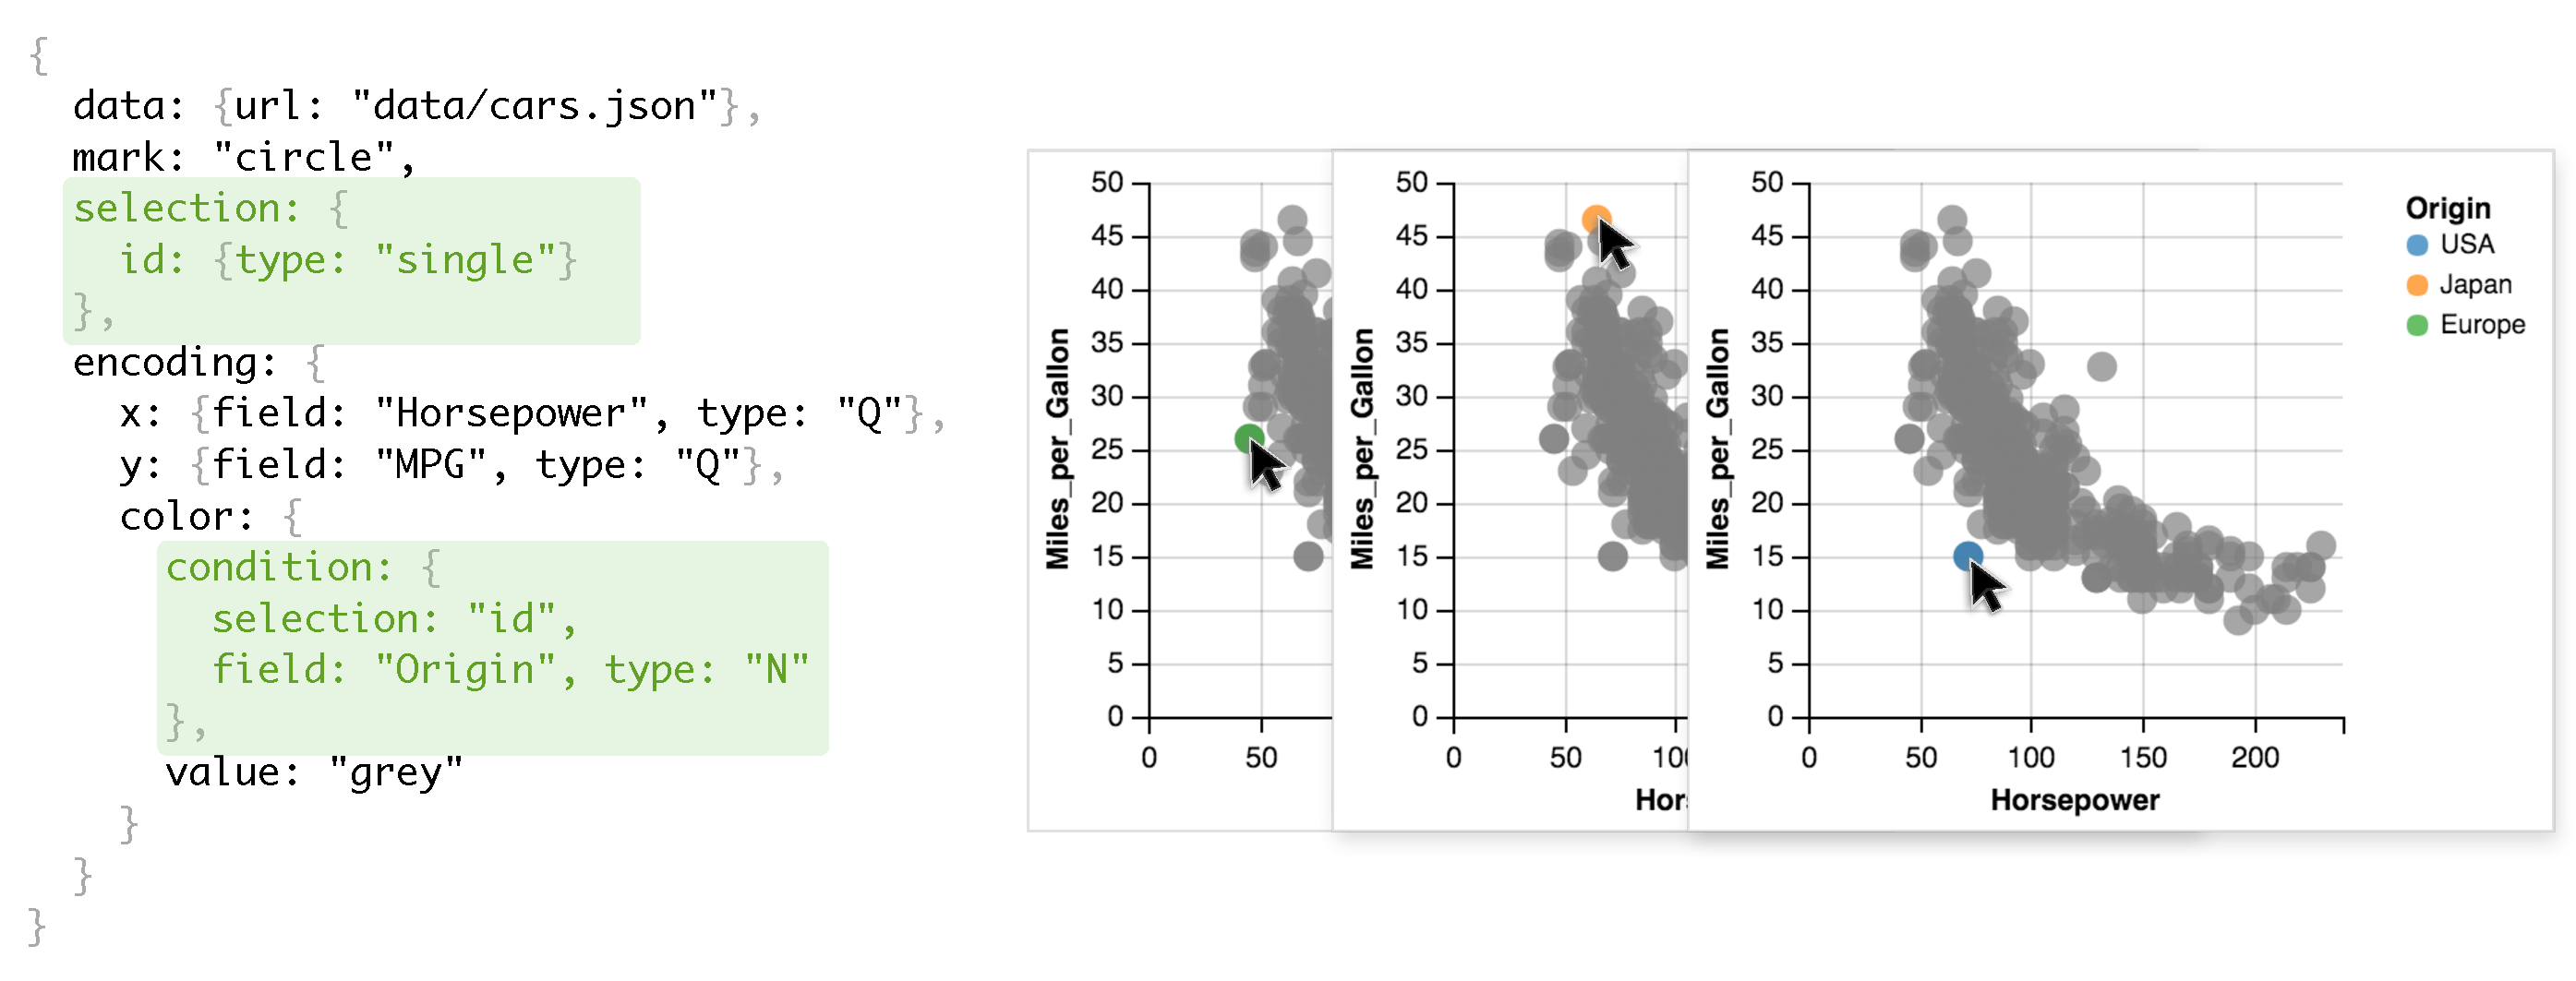
\includegraphics[width=\columnwidth]{singleSelection}
  \caption{Adding a \emph{single} selection to parameterize the fill color
  of a scatterplot's circle mark.}
  \label{fig:vl:singleSelection}
\end{figure*}

\begin{figure*}[h!]
  \centering
  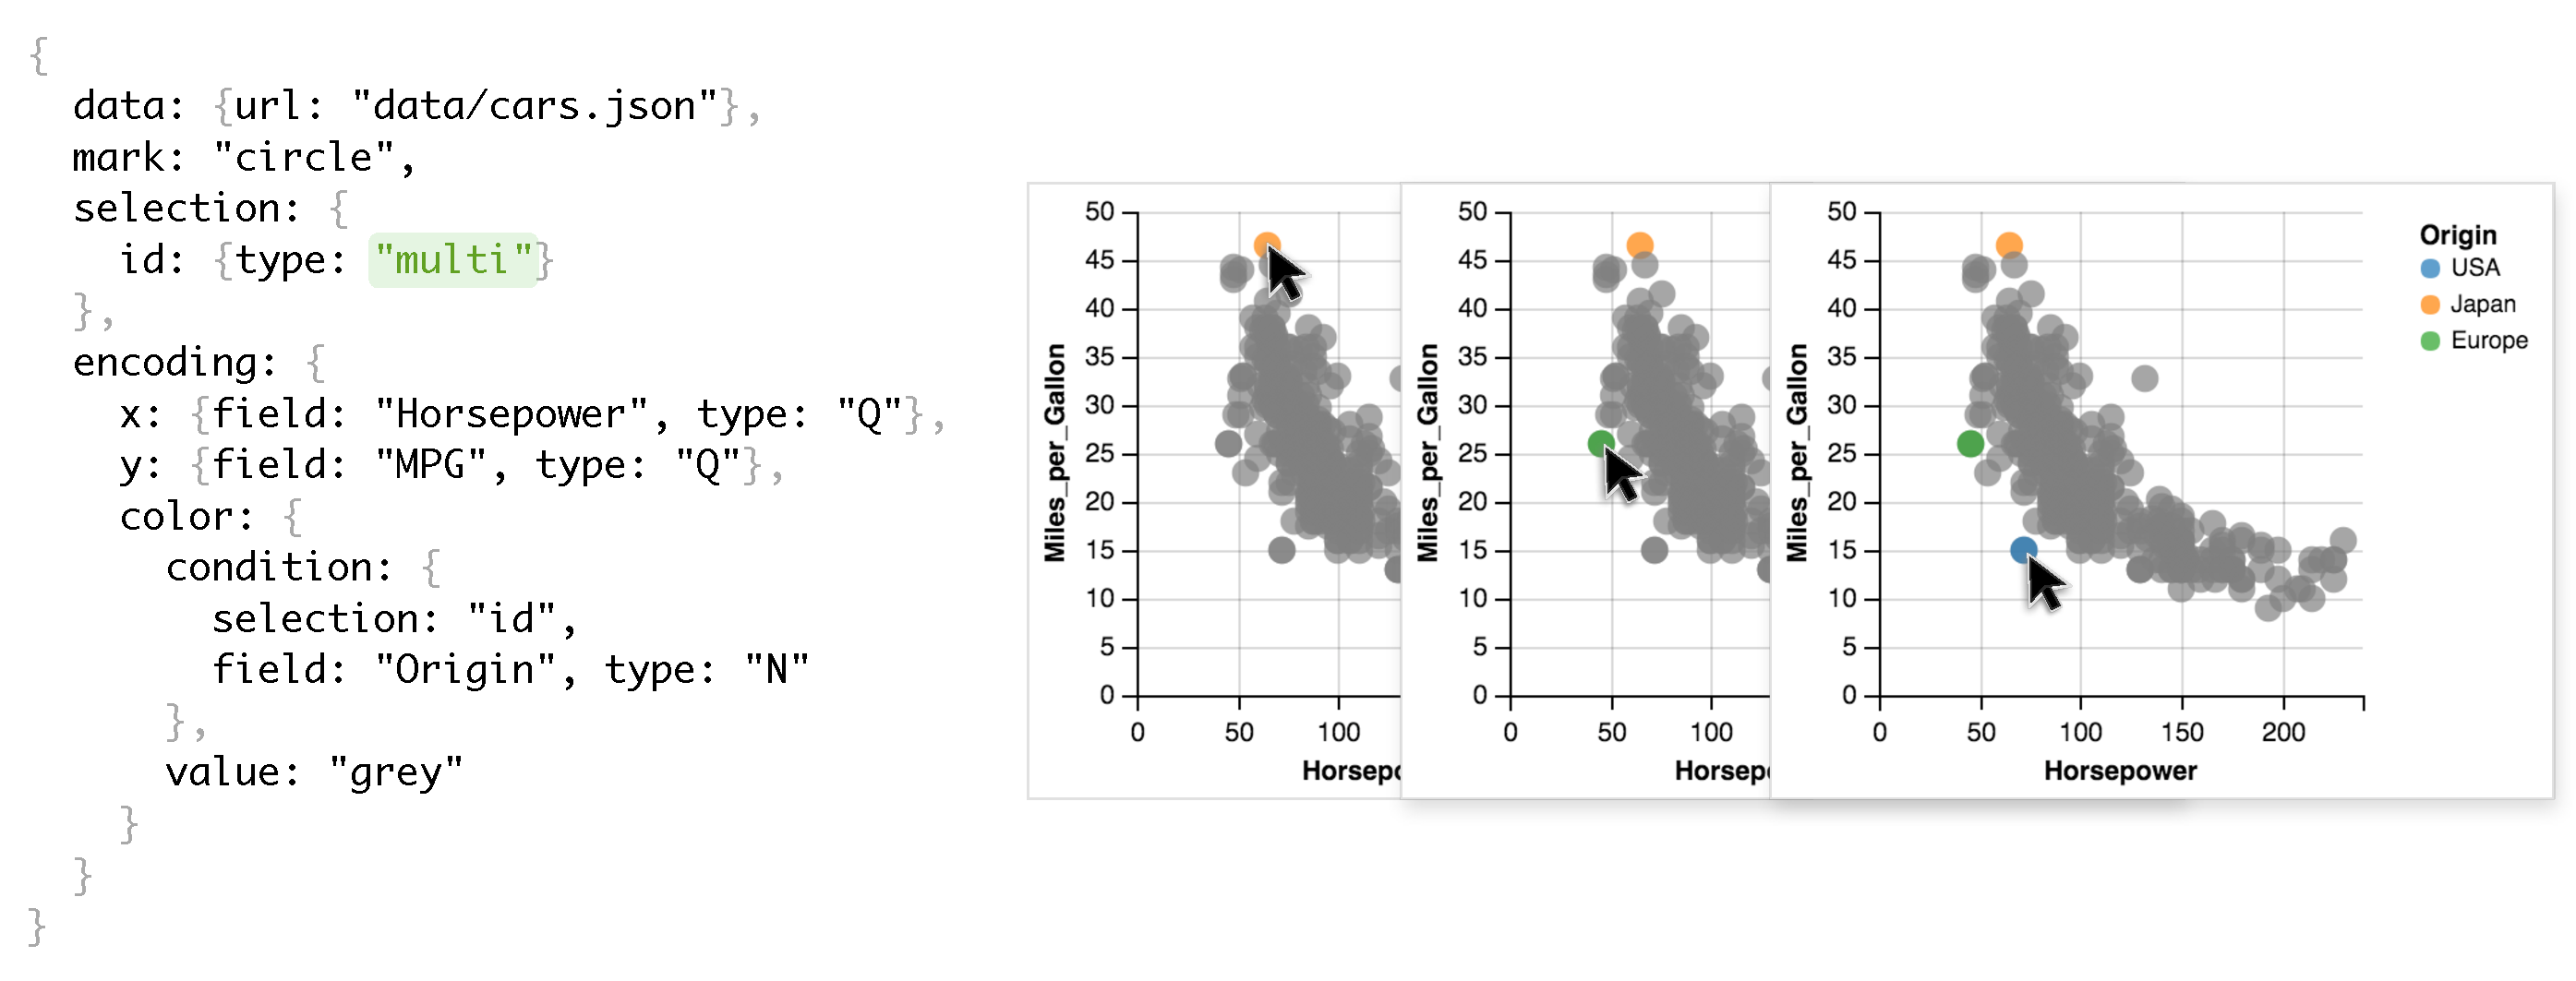
\includegraphics[width=\columnwidth]{multiSelection}
  \caption{Switching from a \emph{single} to \emph{multi} selection. The first
  value is selected on click, and additional values on shift-click.}
  \label{fig:vl:multiSelection}
\end{figure*}

\begin{figure*}[h!]
  \centering
  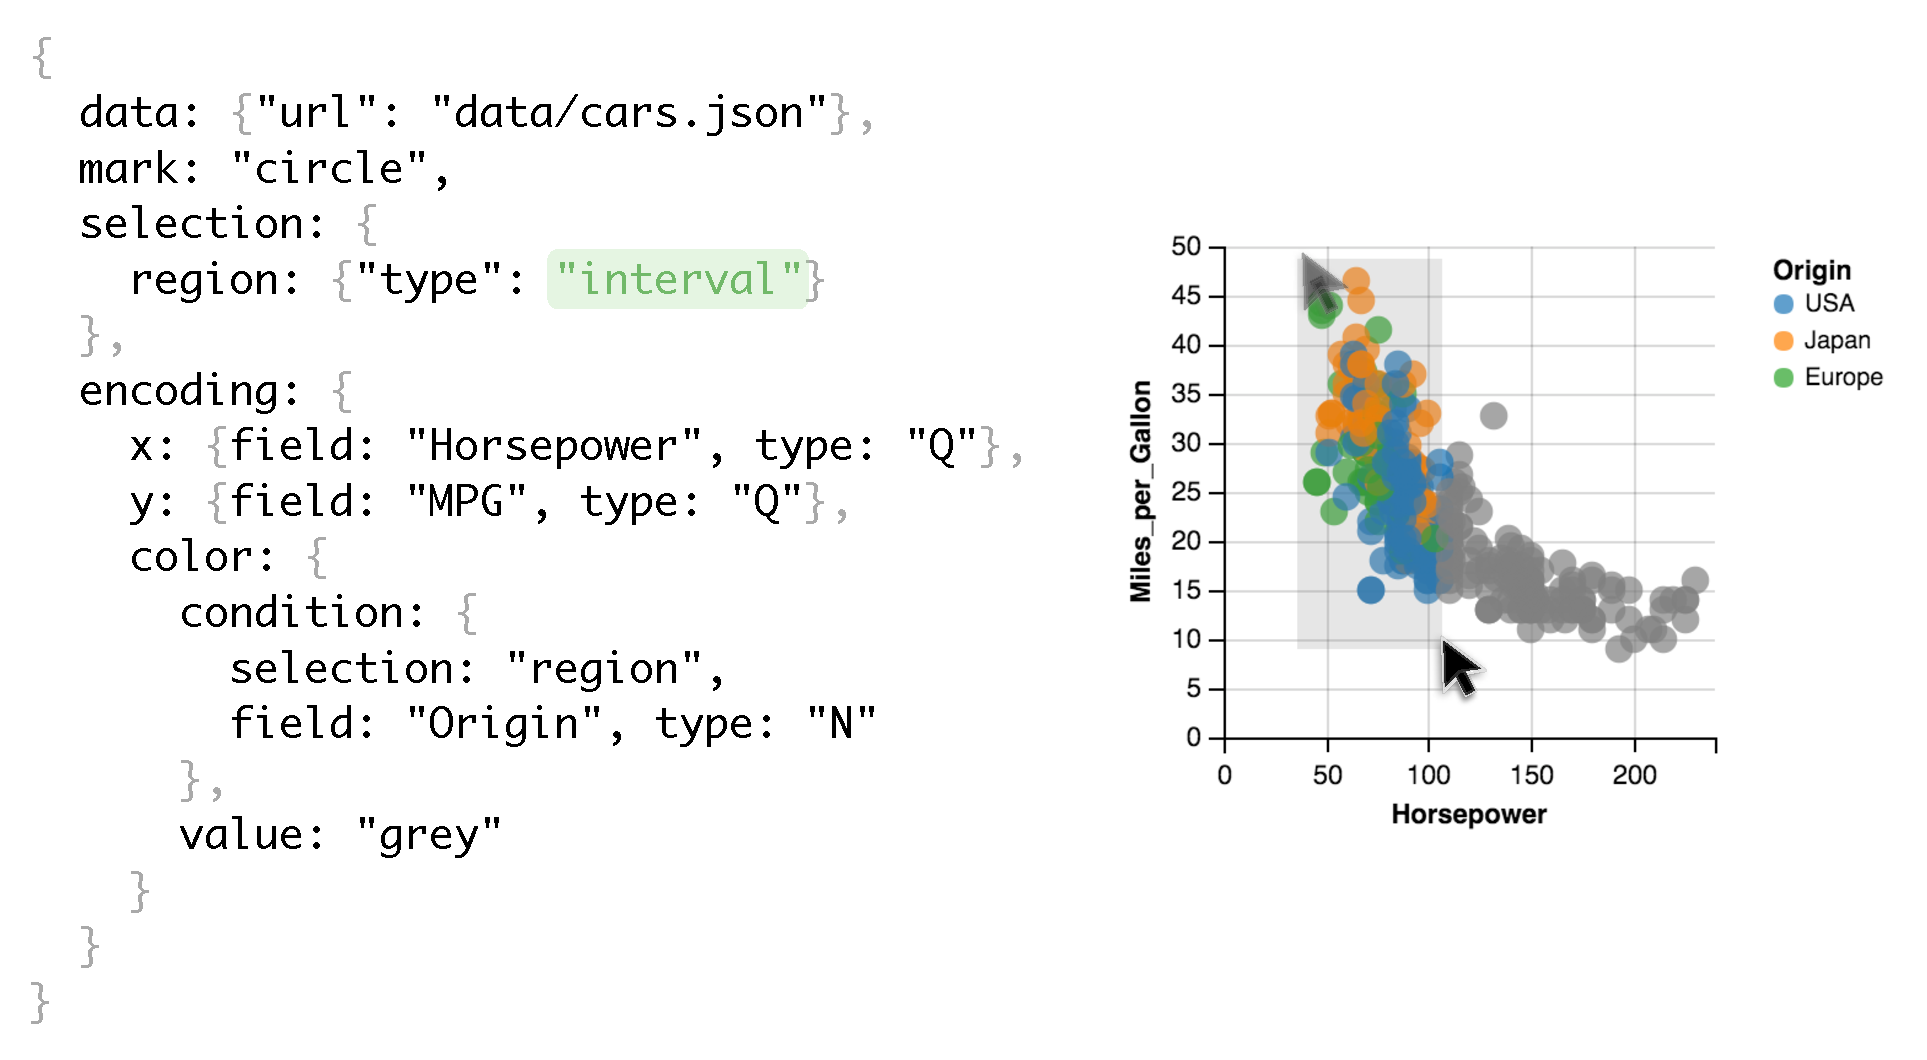
\includegraphics[width=0.8\columnwidth]{intervalSelection}
  \caption{Highlight a continuous range of points using an \emph{interval}
  selection. A rectangle mark is automatically added to depict the interval
  extents.}
  \label{fig:vl:intervalSelection}
\end{figure*}

Predicate functions enable a minimal set of backing points to represent the full
space of selected points. For example, with predicates, an interval selection
need only be backed by two points: the minimum and maximum values of the
interval. While selection types provide default definitions, predicates can be
customized to concisely specify an expressive space of selections. For example,
a single selection with a custom predicate of the form
\texttt{datum.binned\_price == selection.binned\_price} is sufficient for
selecting all data points that fall within a given bin.

By default, backing points lie in the data \emph{domain}. For example, if the
user clicks a mark instance, the underlying data tuple is added to the
selection. If no tuple is available, event properties are passed through inverse
scale transforms. For example, as the user moves their mouse within the data
rectangle, the mouse position is inverted through the \texttt{x} and \texttt{y}
scales and stored in the selection. Defining selections over data values, rather
than visual properties, facilitates reuse across distinct views; each view may
have different encodings specified, but are likely to share the same data
domain. However, some interactions are inherently about manipulating visual
properties\,---\,for example, interactively selecting the colors of a heatmap.
For such cases, users can define selections over the visual \emph{range}
instead. When input events occur, visual elements or event properties are then
stored.

The particular events that update a selection are determined by the platform a
Vega-Lite specification is compiled on, and the input modalities it supports. By
default we use mouse events on desktops, and touch events on mobile and tablet
devices. A user can specify alternate events using Vega's event selectors
(\secref{sec:vg:events}). For example, \cref{fig:vl:paintbrush} demonstrates how
\texttt{mouseover} events are used to populate a multi selection. With the event
selector syntax, multiple events are specified using a comma (e.g.,
\texttt{mousedown, mouseup} adds items to the selection when either event
occurs). A sequence of events is denoted with the between-filter. For example,
\texttt{[mousedown, mouseup] > mousemove} selects all \texttt{mousemove} events
that occur between a \texttt{mousedown} and a \texttt{mouseup} (otherwise known
as ``drag'' events). Events can also be filtered using square brackets (e.g.,
\texttt{mousemove [event.pageY > 5]} for events at the top of the page) and
throttled using braces (e.g., \texttt{mousemove\{100\}} populates a selection at
most every 100 milliseconds).

\begin{figure*}[h!]
  \centering
  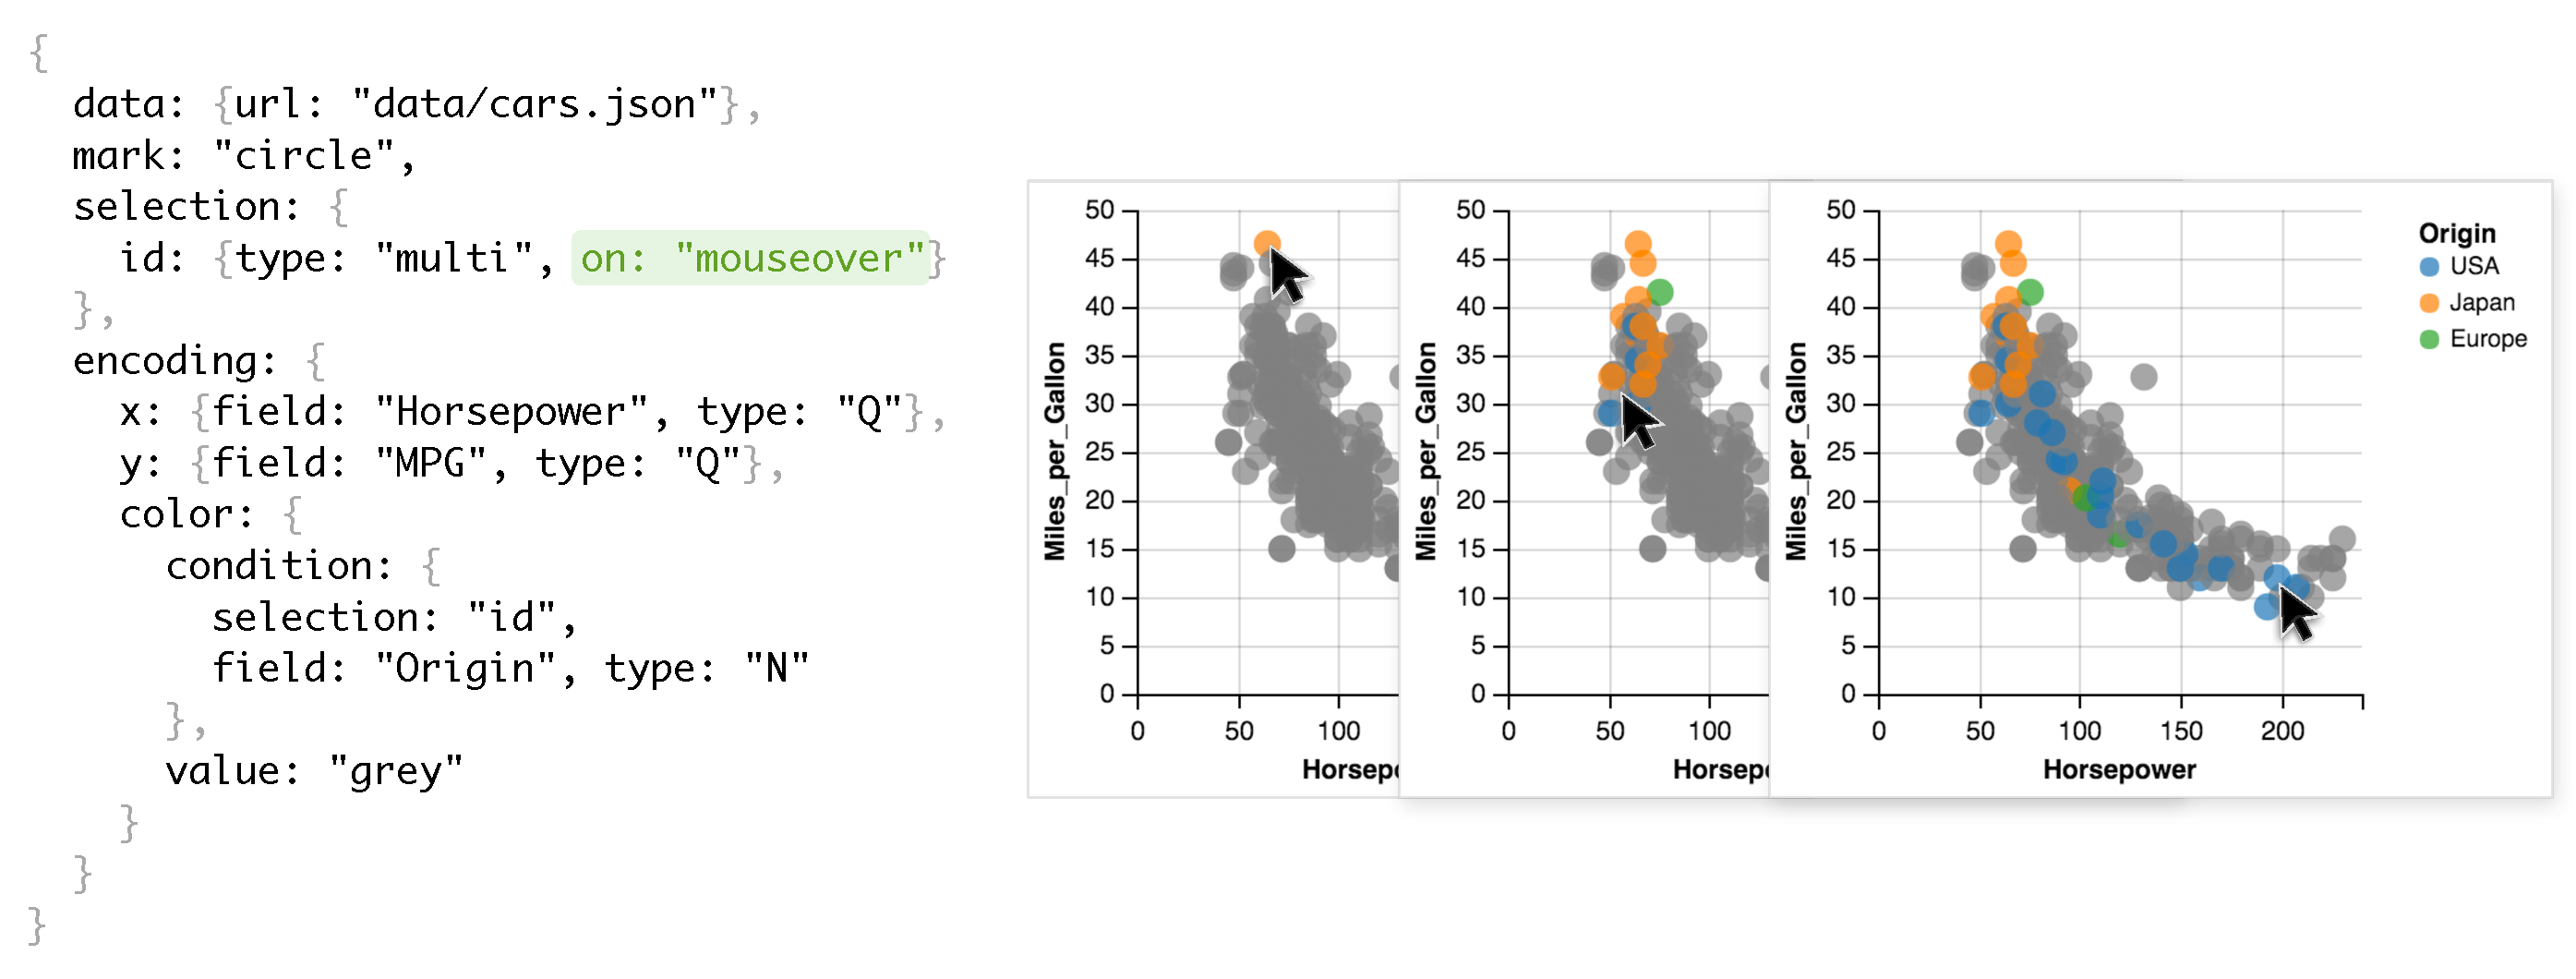
\includegraphics[width=\columnwidth]{paintbrush}
  \caption{Specifying a custom event trigger for a \emph{multi} selection: the
  first point is selected on \texttt{mouseover} and subsequent points when the
  shift key is pressed.}
  \label{fig:vl:paintbrush}
\end{figure*}

\vspace{-10pt}

\subsection{Selection Transforms}

\vspace{-7pt}

Analogous to data transforms, selection transforms manipulate the components of
the selection they are applied to. For example, they may perform operations on
the backing points, alter a selection's predicate function, or modify the input
events that update the selection. Unlike data transforms, however, specifying an
ordering to selection transforms is not necessary as the compilation step
ensures commutativity. All transforms are first parsed, setting properties on an
internal representation of a selection, before they are compiled to produce
event handling and interaction logic.

We identify the following transforms as a minimal set to support both common and
custom interaction techniques. Additional transforms can be defined and
registered with the system, and then invoked within the specification. In this
way, the Vega-Lite language remains concise while ensuring extensibility for
custom behaviors.

% Transforms may be composed\,---\,for
% example, the \emph{toggle} and \emph{nearest} transforms can be applied to a
% multi selection in order to toggle membership of the point nearest the user's
% cursor.

\vspace{-10pt}

\subsubsection{Project}

\vspace{-7pt}

\centerline{\emph{project(fields, channels)}}

The \emph{project} transform alters a selection's predicate function to
determine inclusion by matching only the given \emph{fields}. Some fields,
however, may be difficult for users to address directly (e.g., new fields
introduced due to inline binning or aggregation). For such cases, a list of
\emph{channels} may also be specified (e.g., \texttt{color}, \texttt{size}).

\begin{figure}[h!]
  \centering
  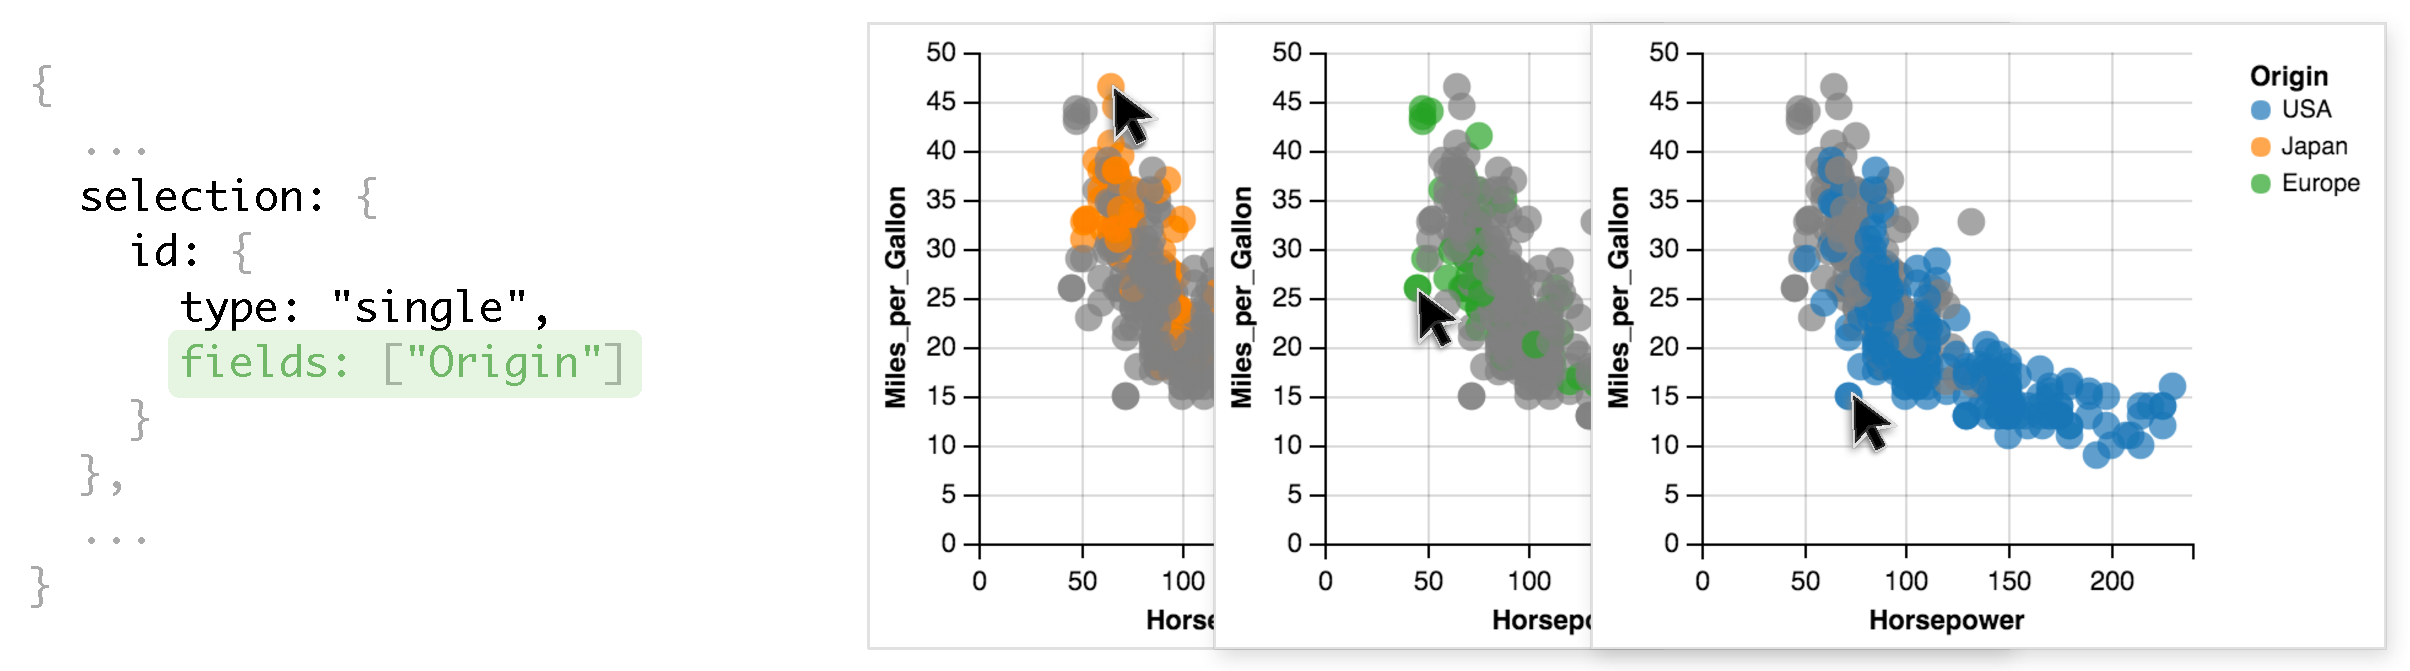
\includegraphics[width=\columnwidth]{projectSingle}
  \caption{Using the \emph{project} transform to highlight a \emph{single}
  \texttt{Origin}.}
  \label{fig:vl:projectSingle}
\end{figure}

\begin{figure}[h!]
  \centering
  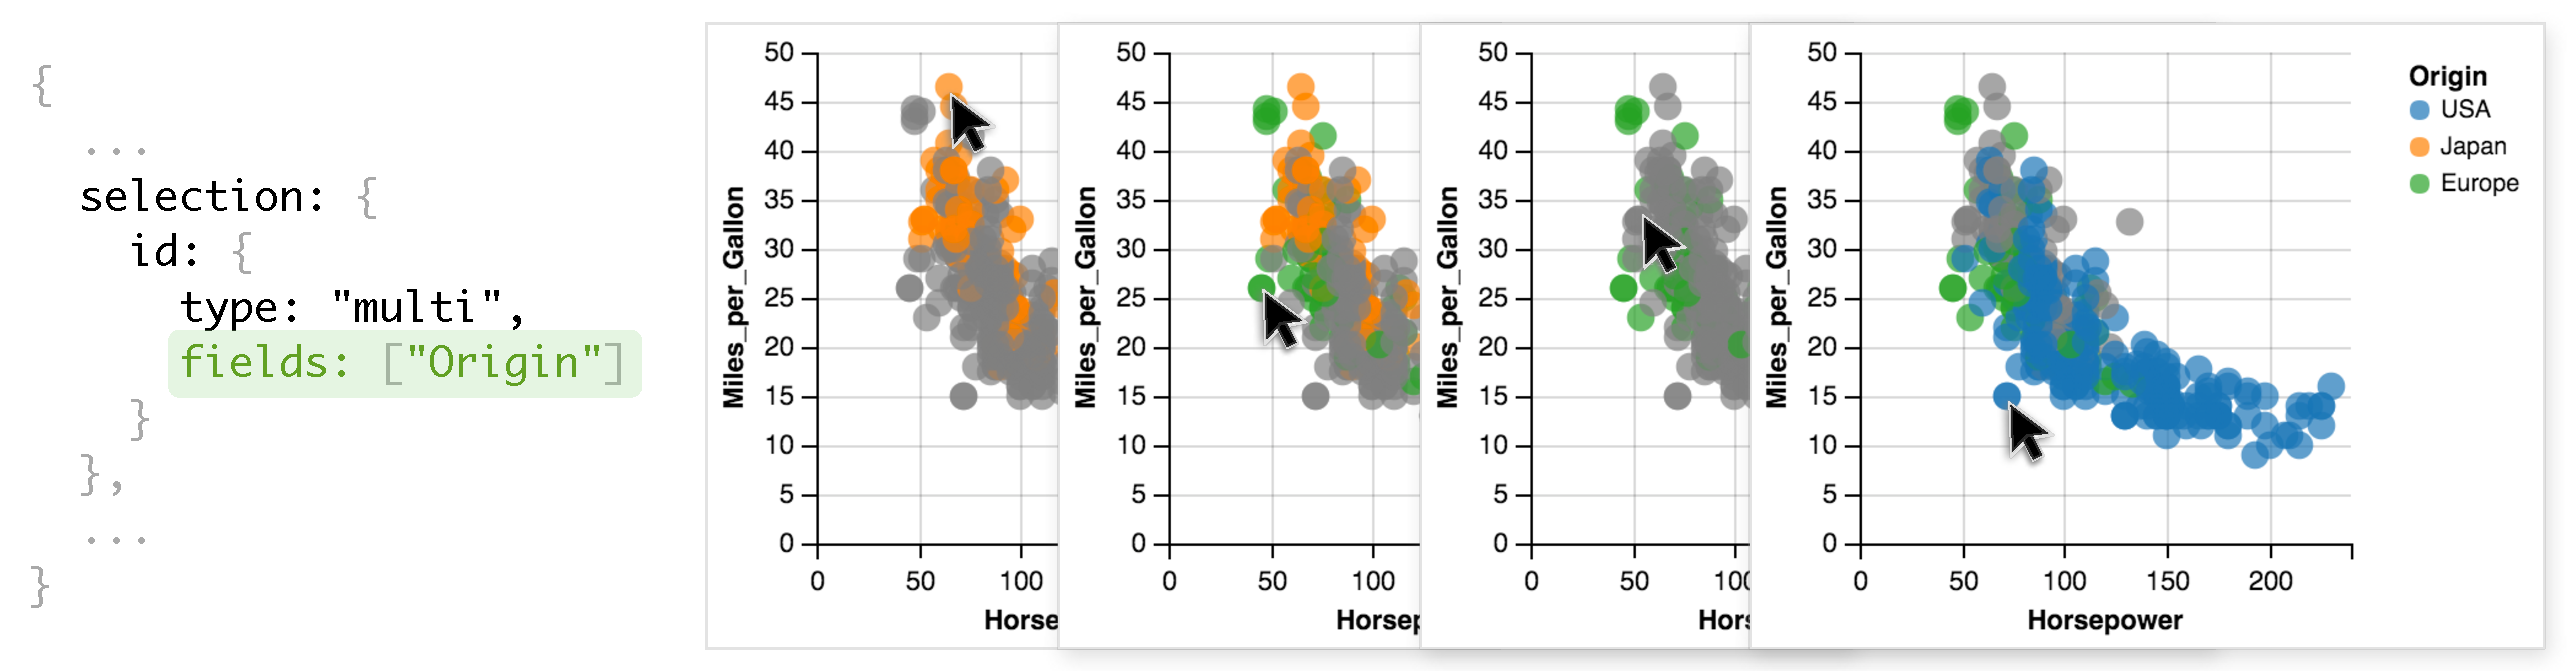
\includegraphics[width=\columnwidth]{projectMulti}
  \caption{Using the \emph{project} transform to highlight \emph{multiple}
  \texttt{Origin}s.}
  \label{fig:vl:projectMulti}
\end{figure}

\begin{figure}[h!]
  \centering
  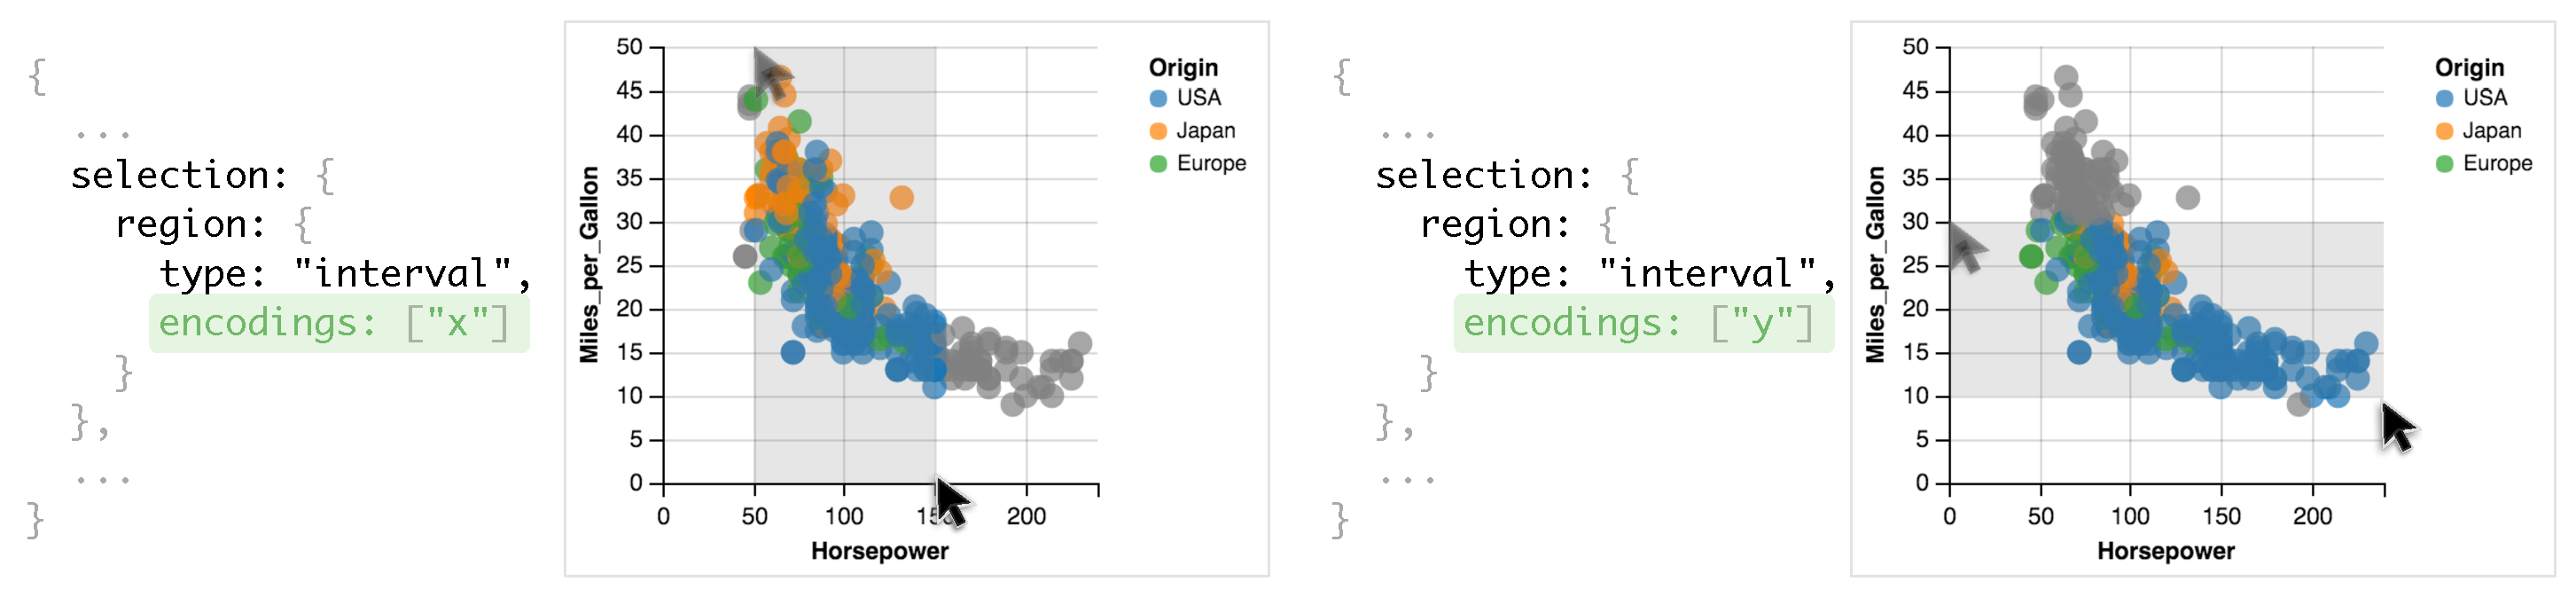
\includegraphics[width=\columnwidth]{projectInterval}
  \caption{\emph{Projecting} an interval selection to restrict it to a
  single dimension.}
  \label{fig:vl:projectInterval}
\end{figure}

\subsubsection{Toggle}

\vspace{-7pt}

\centerline{\emph{toggle(event)}}

The \emph{toggle} transform is automatically instantiated for uninitialized
multi selections. When the \emph{event} occurs, the corresponding data value is
added or removed from the multi selection's backing dataset. By default, the
toggle \emph{event} corresponds to the selection's triggering event, but with
the shift key pressed. For example, in \cref{fig:vl:multiSelection}, additional
points are added to the multi selection on shift-click (where \texttt{click} is
the default event for multi selections). The selection in \cref{fig:vl:paintbrush},
however, specifies a custom \texttt{mouseover} event. Thus, additional points
are inserted when the shift key is pressed and the mouse cursor hovers over a
point.

\vspace{-10pt}

\subsubsection{Translate}

\vspace{-7pt}

\centerline{\emph{translate(events, by)}}

The \emph{translate} transform offsets the spatial properties (or corresponding
data fields) of backing points by an amount determined by the coordinates of the
sequenced \emph{events}. For example, on the desktop, drag events
(\texttt{[mousedown, mouseup] > mousemove}) are used and the offset corresponds
to the difference between where the \texttt{mousedown} and subsequent
\texttt{mousemove} events occur. If no coordinates are available (e.g., as with
keyboard events), a \emph{by} argument should be specified. This transform
respects the \emph{project} transform as well, restricting movement to the
specified dimensions. This transform is automatically instantiated for interval
selections.

\begin{figure}[h!]
  \centering
  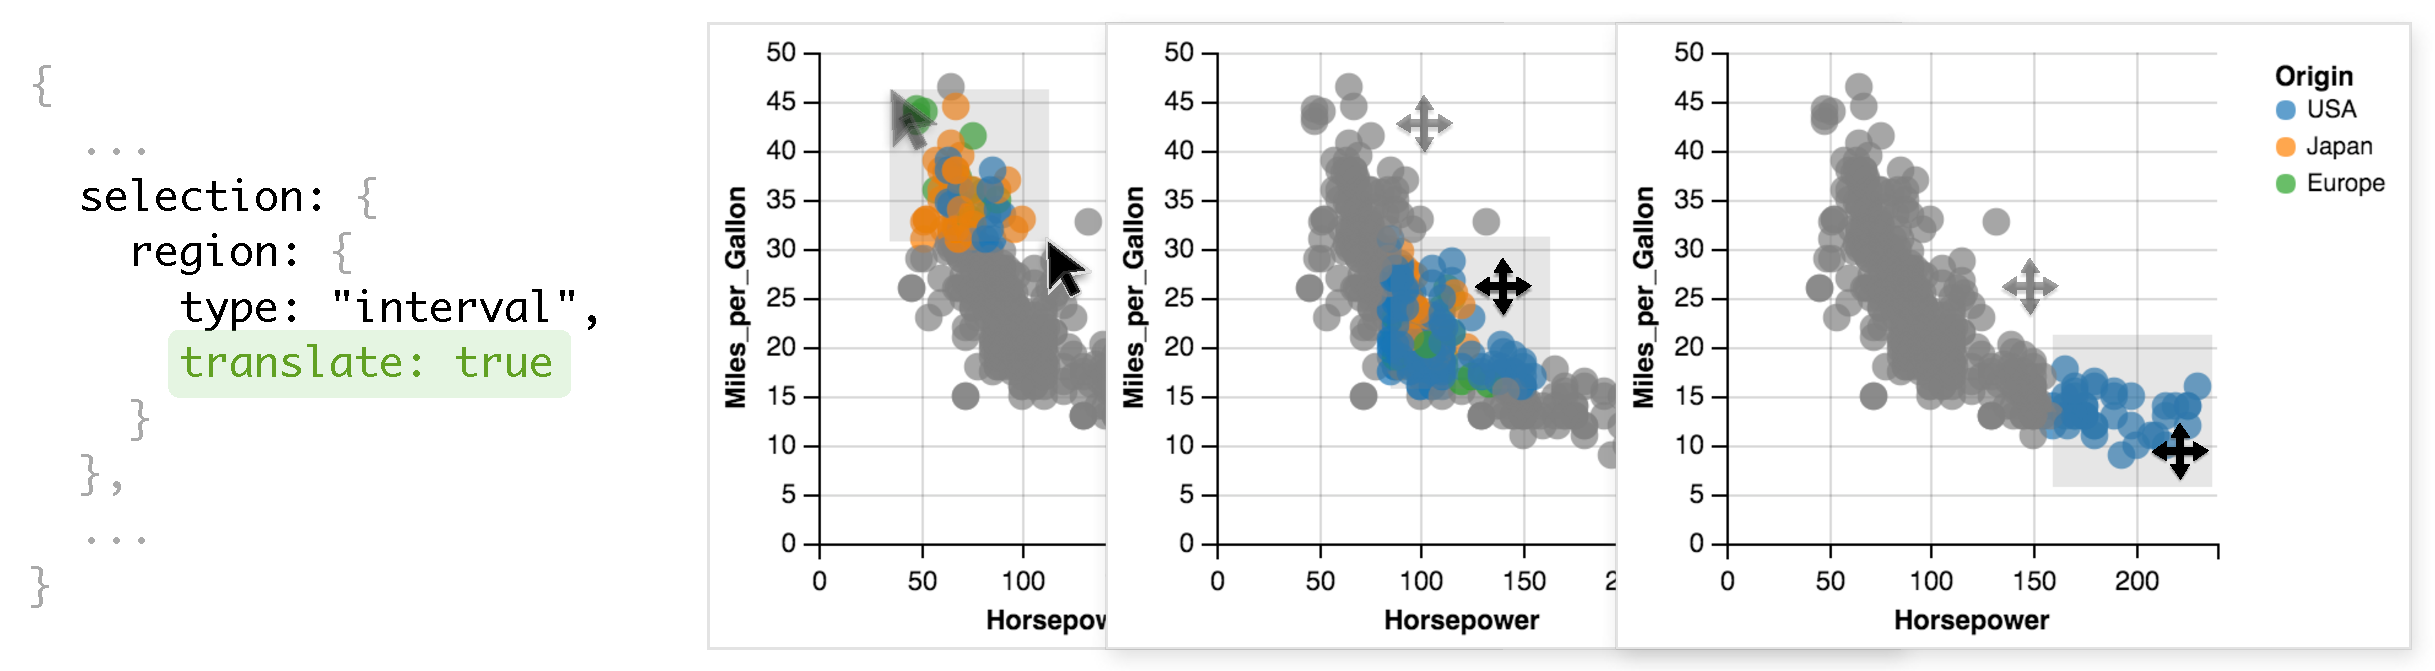
\includegraphics[width=\columnwidth]{translate}
  \caption{The \emph{translate} transform enables movement of the brushed
  region. It is automatically invoked for interval selections but is
  explicitly depicted here for clarity.}
  \label{fig:vl:translate}
\end{figure}

\subsubsection{Zoom}

\vspace{-7pt}

\centerline{\emph{zoom(event, factor)}}

The \emph{zoom} transform applies a scale factor, determined by the \emph{event}
to the spatial properties (or corresponding data fields) of backing points. A
\emph{factor} must be specified if it cannot be determined from the events
(e.g., when arrow keys are pressed). When combined with the \emph{project}
transform, an interval can be zoomed uni-dimensionally.

\vspace{-10pt}

\subsubsection{Bind}

\vspace{-7pt}

\centerline{\emph{bind(widgets$|$scales)}}

The \emph{bind} transform establishes a two-way binding between control widgets
(e.g., sliders, textboxes, etc.) or scale functions for single and interval
selections respectively.

When a single selection is bound to query widgets, one widget per projected
field is generated and may be used to manipulate the corresponding predicate
clause. When triggering events occur to update the selected points, the widgets
are updated as well. Control widgets, in addition to direct manipulation
interaction, allow for more rapid and exhaustive querying of the backing
data~\cite{shneiderman:dynamicqueries}. For example, scrubbing a slider back and
forth can quickly reveal a trend in the data or highlight a small number of
selected points that would otherwise be difficult to pick out directly.

Interval selections can be bound to the scales of the unit specification they
are defined in. Doing so \emph{initializes} the selection, populating it with
the given scales' domain or range, and parameterizes the scales to use the
selection instead. Binding selections to scales allows scale extents to be
interactively manipulated, yet remain automatically initialized by the input
data. By default, both the \texttt{x} and \texttt{y} scales are bound; alternate
scales are specified by \emph{projecting} over the corresponding channels.

\begin{figure}[h!]
\floatbox[{\capbeside\thisfloatsetup{capbesideposition=
{right,center},capbesidewidth=0.35\columnwidth}}]{figure}[\FBwidth]
{\caption{Panning and zooming the scatterplot is achieved by first
\emph{binding} an interval selection to the x- and y-scale domains, and then
applying the \emph{translate} and \emph{zoom} transforms. Alternate events
prevent collision with the brushing interaction, previously defined in
\cref{fig:vl:intervalSelection}}
\label{fig:vl:bindScales}}
{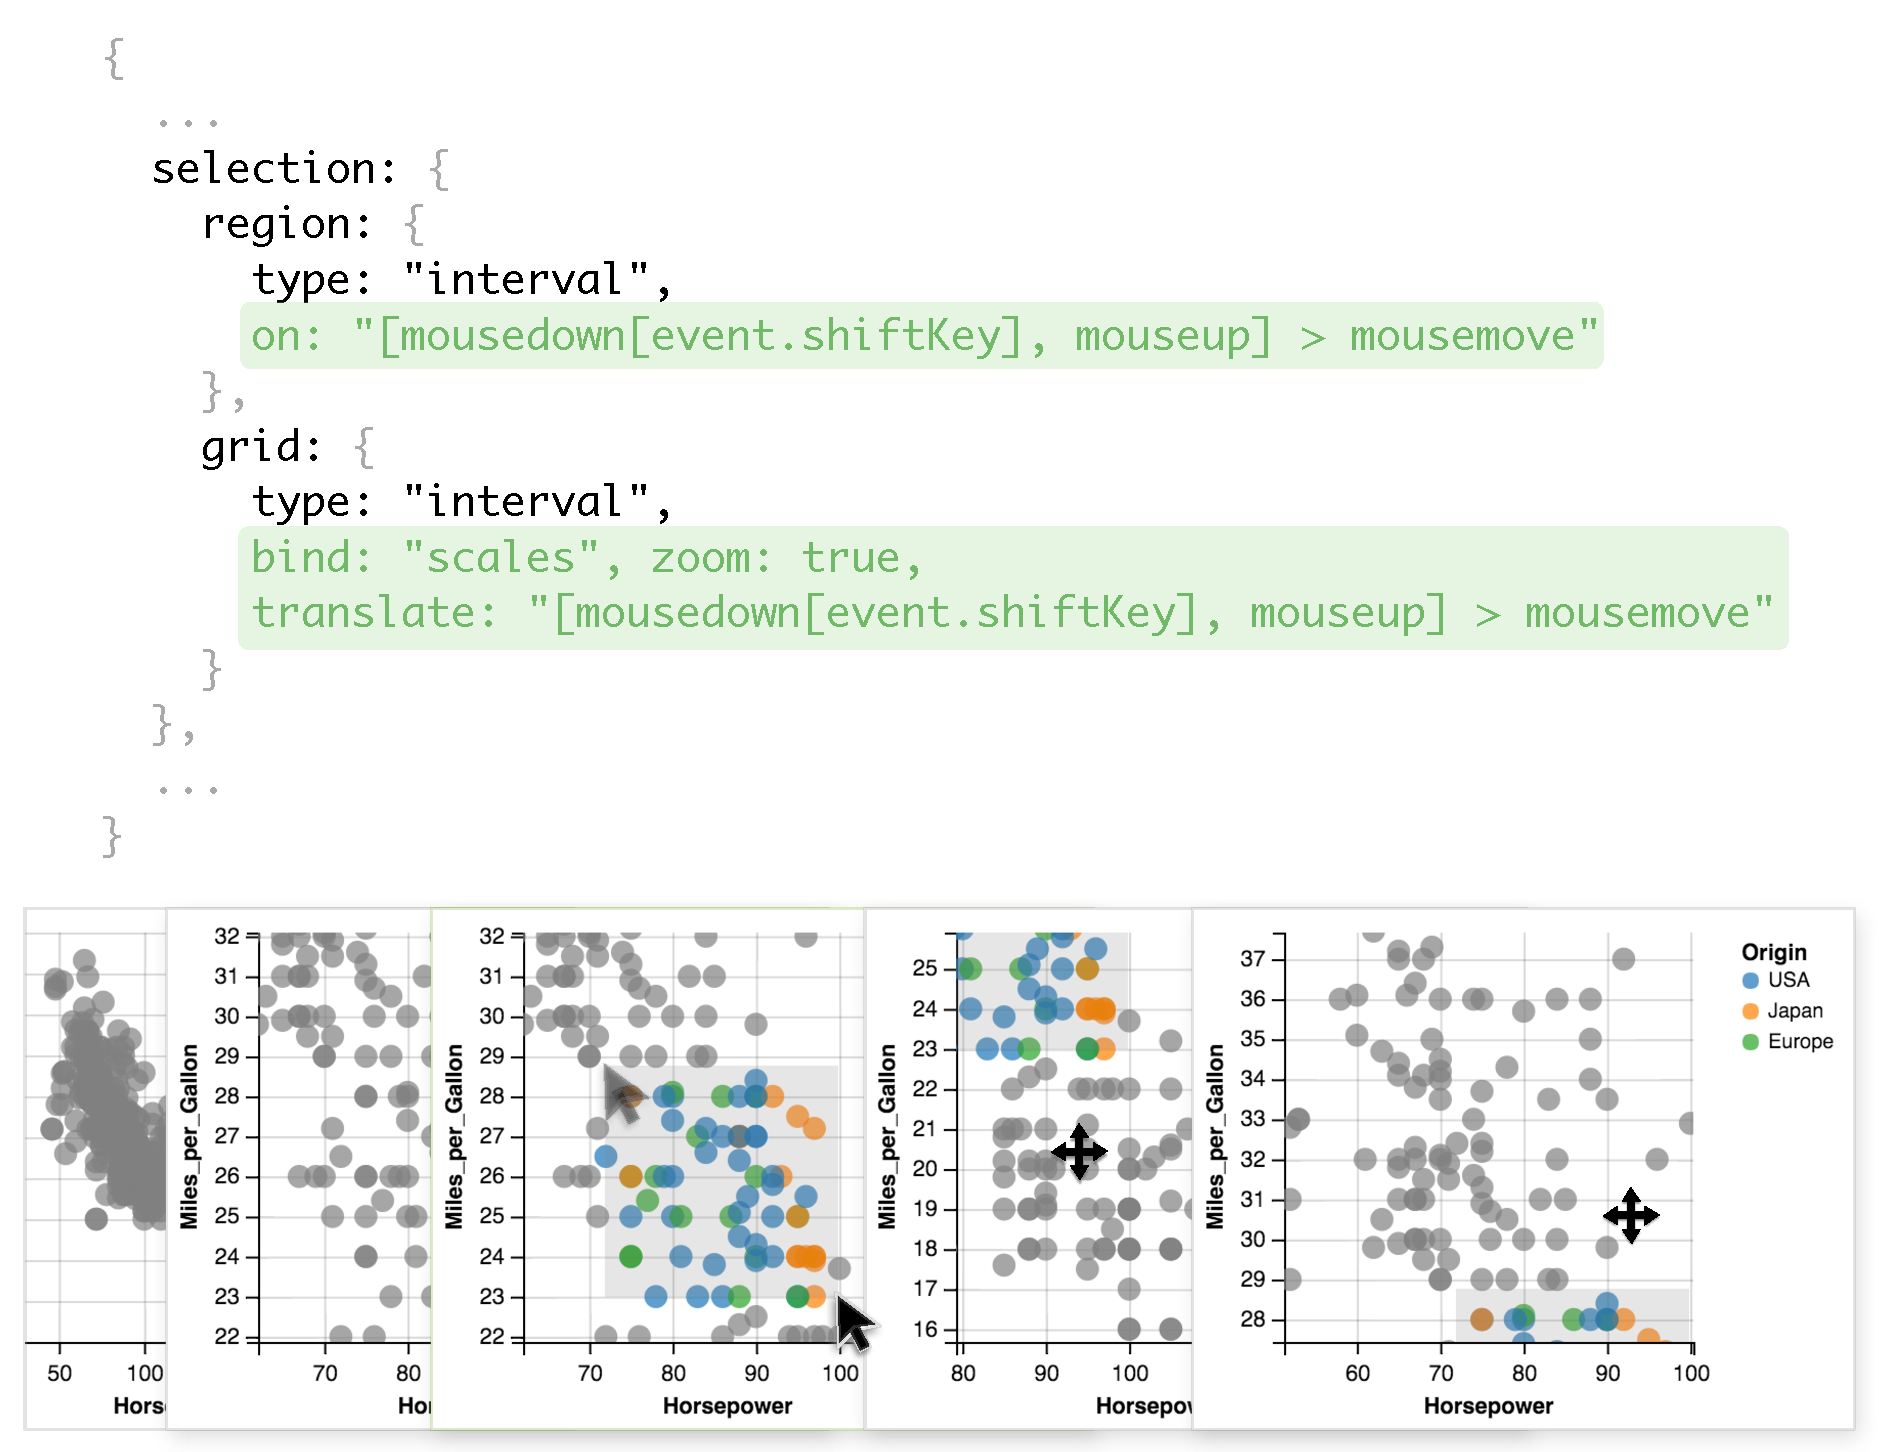
\includegraphics[width=0.65\textwidth]{bindScales}}
\end{figure}

\vspace{-10pt}

\subsubsection{Nearest}

\vspace{-7pt}

\centerline{\emph{nearest()}}

The \emph{nearest} transform computes a Voronoi decomposition, and augments the
selection's event processing. The data value or visual element nearest the
triggering \emph{event} is now selected (approximating a Bubble
Cursor~\cite{grossman:bubble}). Currently, the centroid of each mark instance is
used to calculate the Voronoi diagram but we plan to extend this operator to
account for boundary points as well (e.g., rectangle vertices).

\vspace{-10pt}

\subsection{Selection-Driven Visual Encodings}

\vspace{-7pt}

Once selections are defined, they parameterize visual encodings to make them
interactive\,---\,visual encodings are automatically reevaluated as selections
change. First, selections can be used to drive \emph{conditional} encoding
rules. Each data tuple participating in the encoding is evaluated against the
selection's predicate, and properties are set based on whether it belongs to the
selection or not. For example, as shown in
\cref{fig:vl:singleSelection,fig:vl:multiSelection}, the fill color of the scatterplot
circles is determined by a data field if they fall within the \texttt{id}
selection, or set to grey otherwise.

Next, selected points can be explicitly materialized and used as input data for
other encodings within the specification. By default, this applies a selection's
predicate against the data tuples (or visual elements) of the unit specification
it is defined in. To materialize a selection against an arbitrary dataset, a
\emph{map} transform rewrites the predicate function to account for differing
schemas. Using selections in this way enables linked interactions, including
displaying tooltips or labels, and cross-filtering.

Besides serving as input data, a materialized selection can also define scale
extents. Binding a selection to scales offers a concise way of specifying this
behavior within the same unit specification. For multi-view displays, selection
names can be specified as the domain or range of a particular channel's scale.
Doing so constructs interactions that manipulate viewports, including panning \&
zooming (\cref{fig:vl:bindScales}) and overview\,+\,detail
(\cref{fig:vl:overviewDetail}).

In all three cases, selections can be composed using logical \texttt{OR},
\texttt{AND}, and \texttt{NOT} operators. As previously discussed, single
selections offer an additional mechanism for parameterizing encodings. The
backing point can be directly referenced within the specification, for example
as part of a filter or calculate expression, or to determine a visual encoding
channel without the overhead of a conditional rule. In \cref{fig:vl:indexChart},
for instance, the red rule is positioned using the \texttt{date} value of the
\texttt{indexPt} selection.

\vspace{-10pt}

\subsection{Disambiguating Composite Selections}

\vspace{-7pt}

Selections are defined within unit specifications to provide a default
context\,---\,a selection's events are registered on the unit's mark instances,
and materializing a selection applies its predicate against the unit's input
data by default. When units are composed, however, selection definitions and
applications become ambiguous.

Consider \cref{fig:vl:resolveGlobal}, which illustrates how a scatterplot matrix
(SPLOM) is constructed by repeating a unit specification. To brush, we define an
interval selection (\texttt{region}) within the unit, and use it to perform a
linking operation by parameterizing the color of the circle marks. However,
there are several ambiguities within this setup. Is there one \texttt{region}
for the overall visualization, or one per cell? If the latter, which cell's
\texttt{region} should be used to highlight the points?  This ambiguity recurs
when selections serve as input data or scale extents, and when selections share
the same name across a layered or concatenated views.

\begin{figure}[b!]
  \centering
  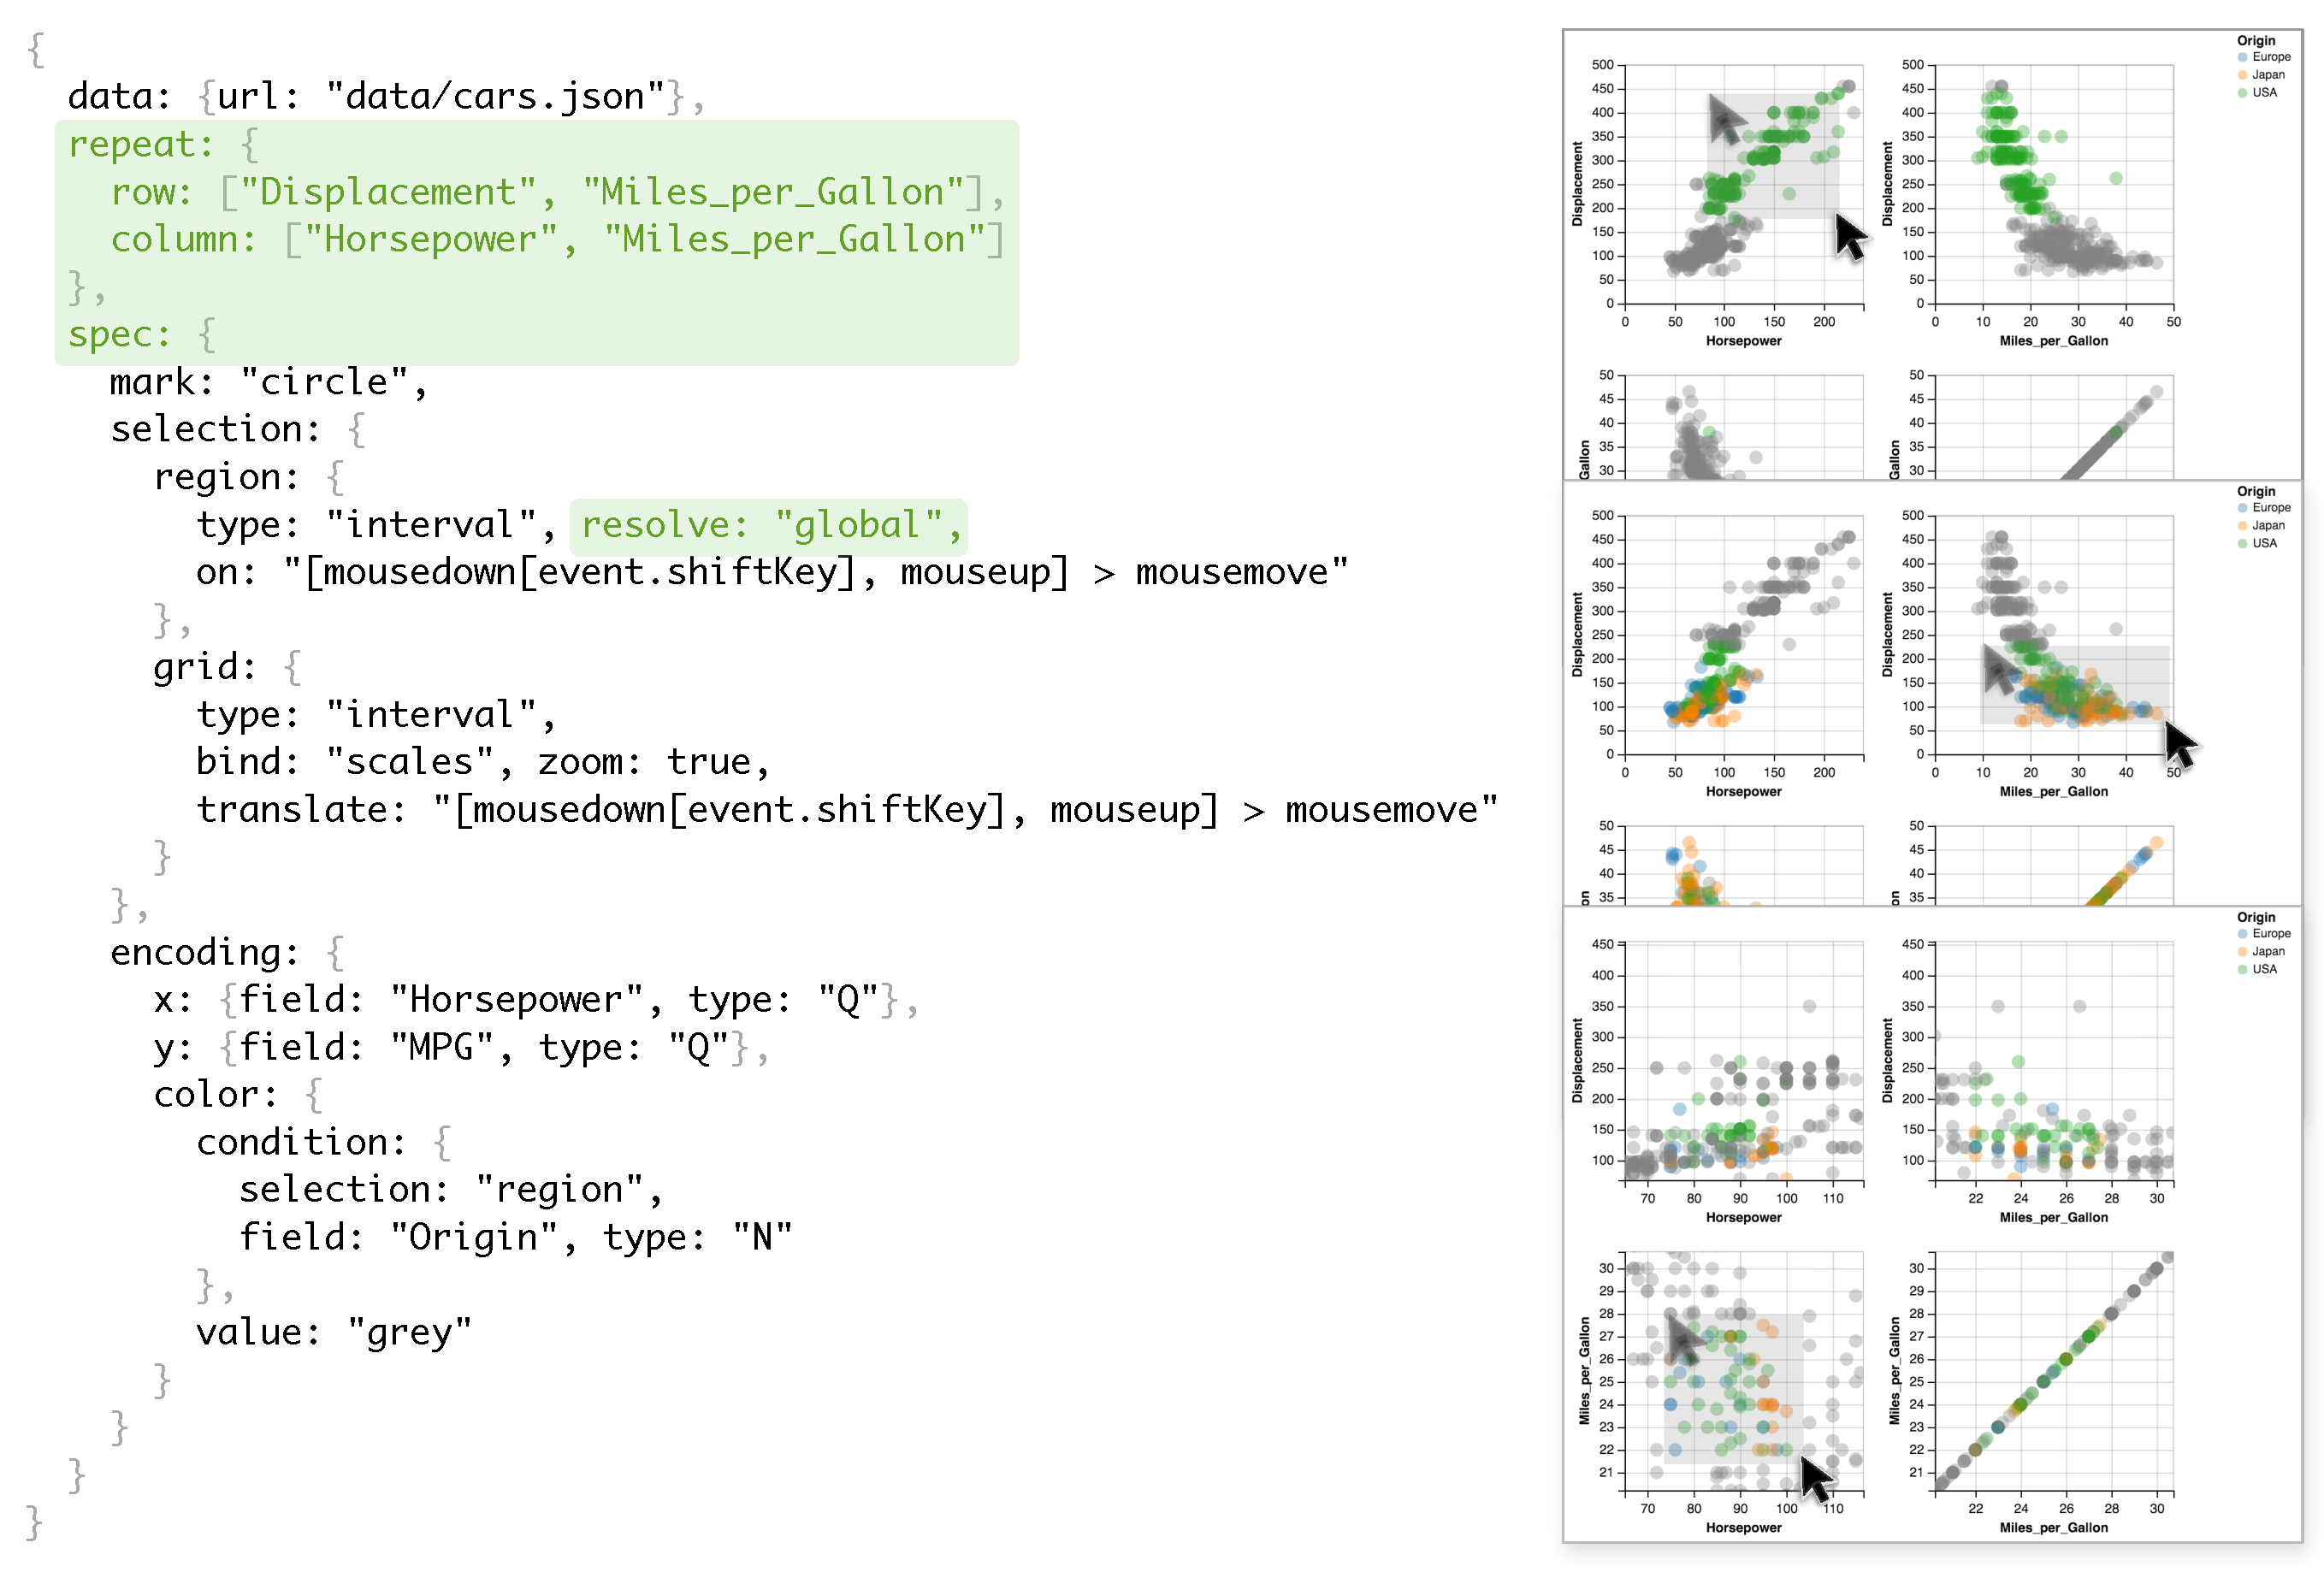
\includegraphics[width=\columnwidth]{resolveGlobal}
  \caption{By adding a \emph{repeat} operator, we compose the encodings and
  interactions from \cref{fig:vl:bindScales} into a scatterplot matrix. Users can
  brush, pan, and zoom within each cell, and the others update in concert. By
  default, a \emph{global} composite selection is created: brushing in a cell
  replaces previous brushes.}
  \label{fig:vl:resolveGlobal}
\end{figure}

Several strategies exist for resolving this ambiguity. By default, a
\emph{global} selection exists across all views. With our SPLOM example, this
setting causes only one brush to be populated and shared across all cells. When
the user brushes in a cell, points that fall within it are highlighted, and
previous brushes are removed.

Users can specify an alternate ambiguity resolution when defining a selection.
These schemes all construct one instance of the selection per view, and define
which instances are used in determining inclusion. For example, resolving a
selection to \emph{independent} creates one instance per view, and each unit
uses only its own selection to determine inclusion. With our SPLOM example, this
would produce the interaction shown below. Each cell would display its own
brush, which would determine how only its points would be highlighted.

Selections can also be resolved to \emph{union} or \emph{intersect}. Here, all
instances of a selection are considered in concert: a point falls within the
overall selection if it is included in, respectively, at least one of the
constituents or all of them. More concretely, with the SPLOM example, these
settings would continue to produce one brush per cell, and points would
highlight when they lie within at least one brush (\emph{union}) or if they are
within every brush (\emph{intersect}) as shown in
\cref{fig:vl:resolveUnion,fig:vl:resolveIntersect} respectively. We also support
\emph{union others} and \emph{intersect others} resolutions, which function like
their full counterparts except that a unit's own selection is not part of the
inclusion determination. These latter methods support cross-filtering
(\cref{fig:vl:crossfilter}) where interactions within a view should not filter
itself.

\begin{figure}[h!]
  \centering
  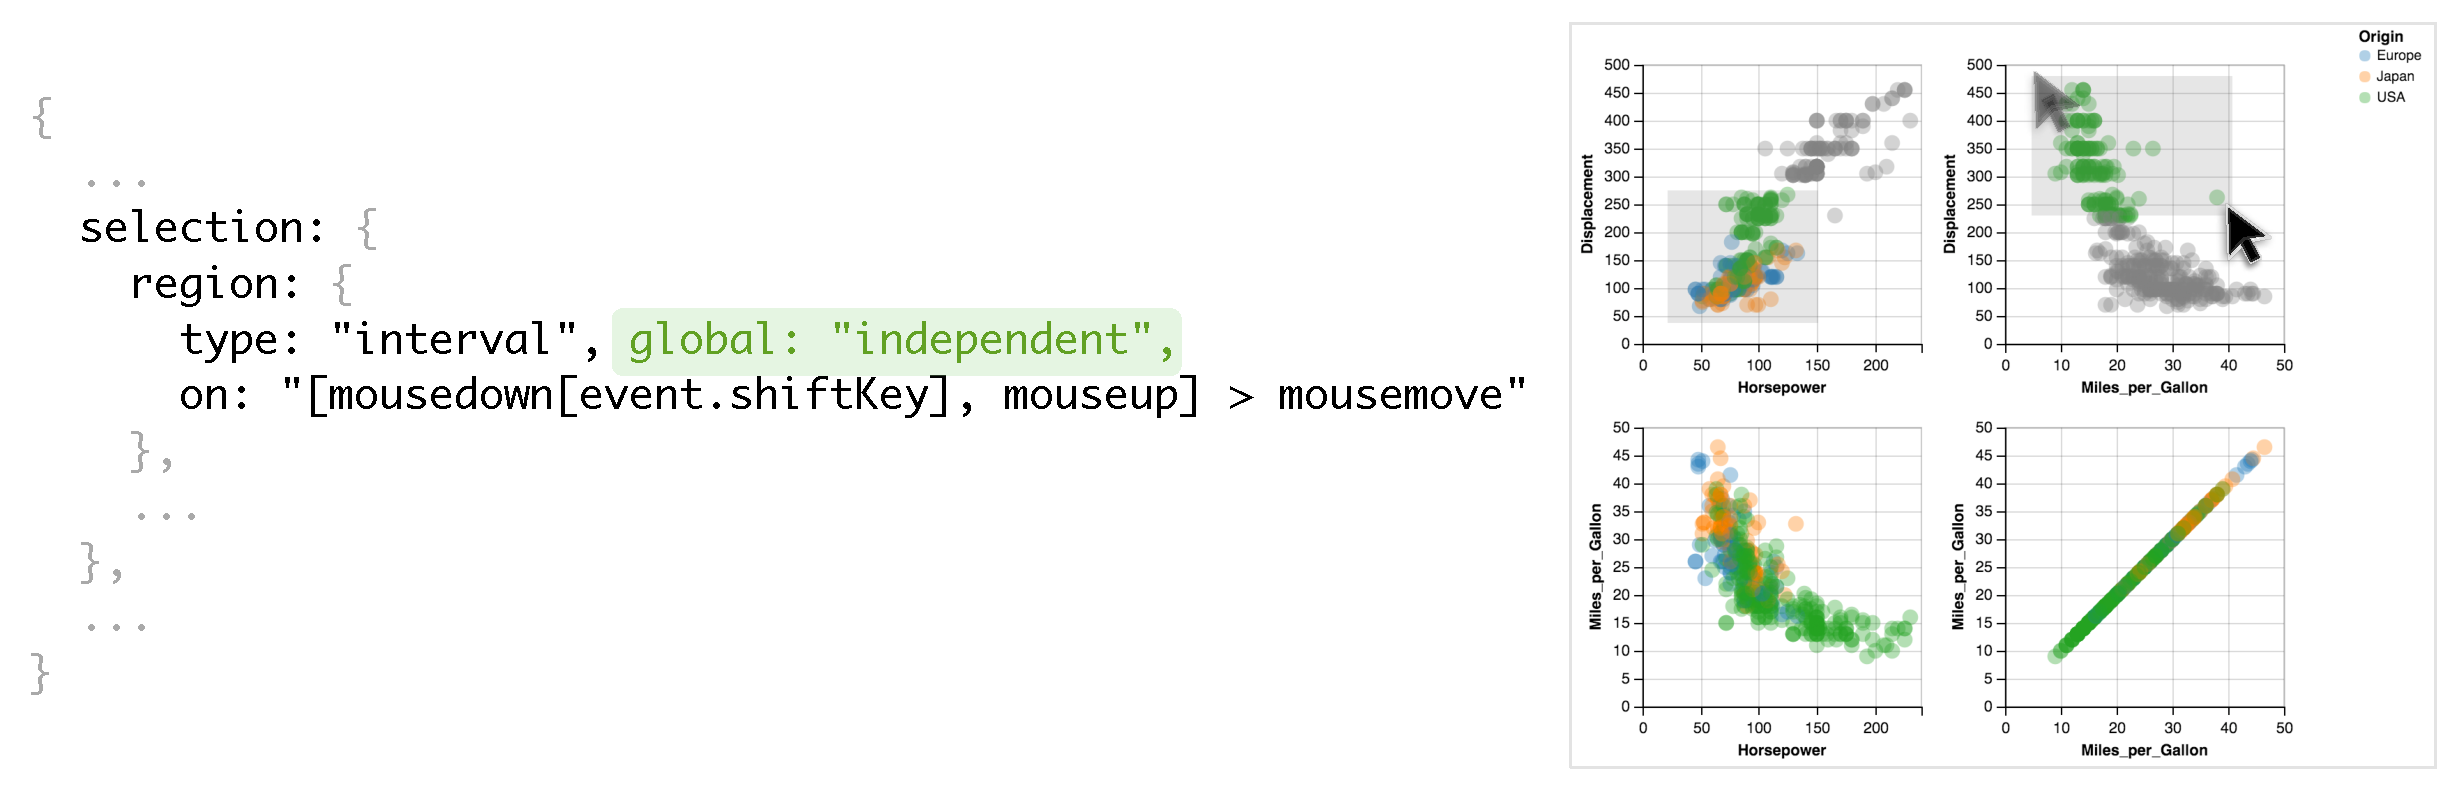
\includegraphics[width=\columnwidth]{resolveIndependent}
  \caption{Resolving the \texttt{region} selection to \emph{independent}
produces a brush in each cell, and points only highlight based on the selection
in their own cell.}
  \label{fig:vl:resolveIndependent}
\end{figure}

\begin{figure}[h!]
  \centering
  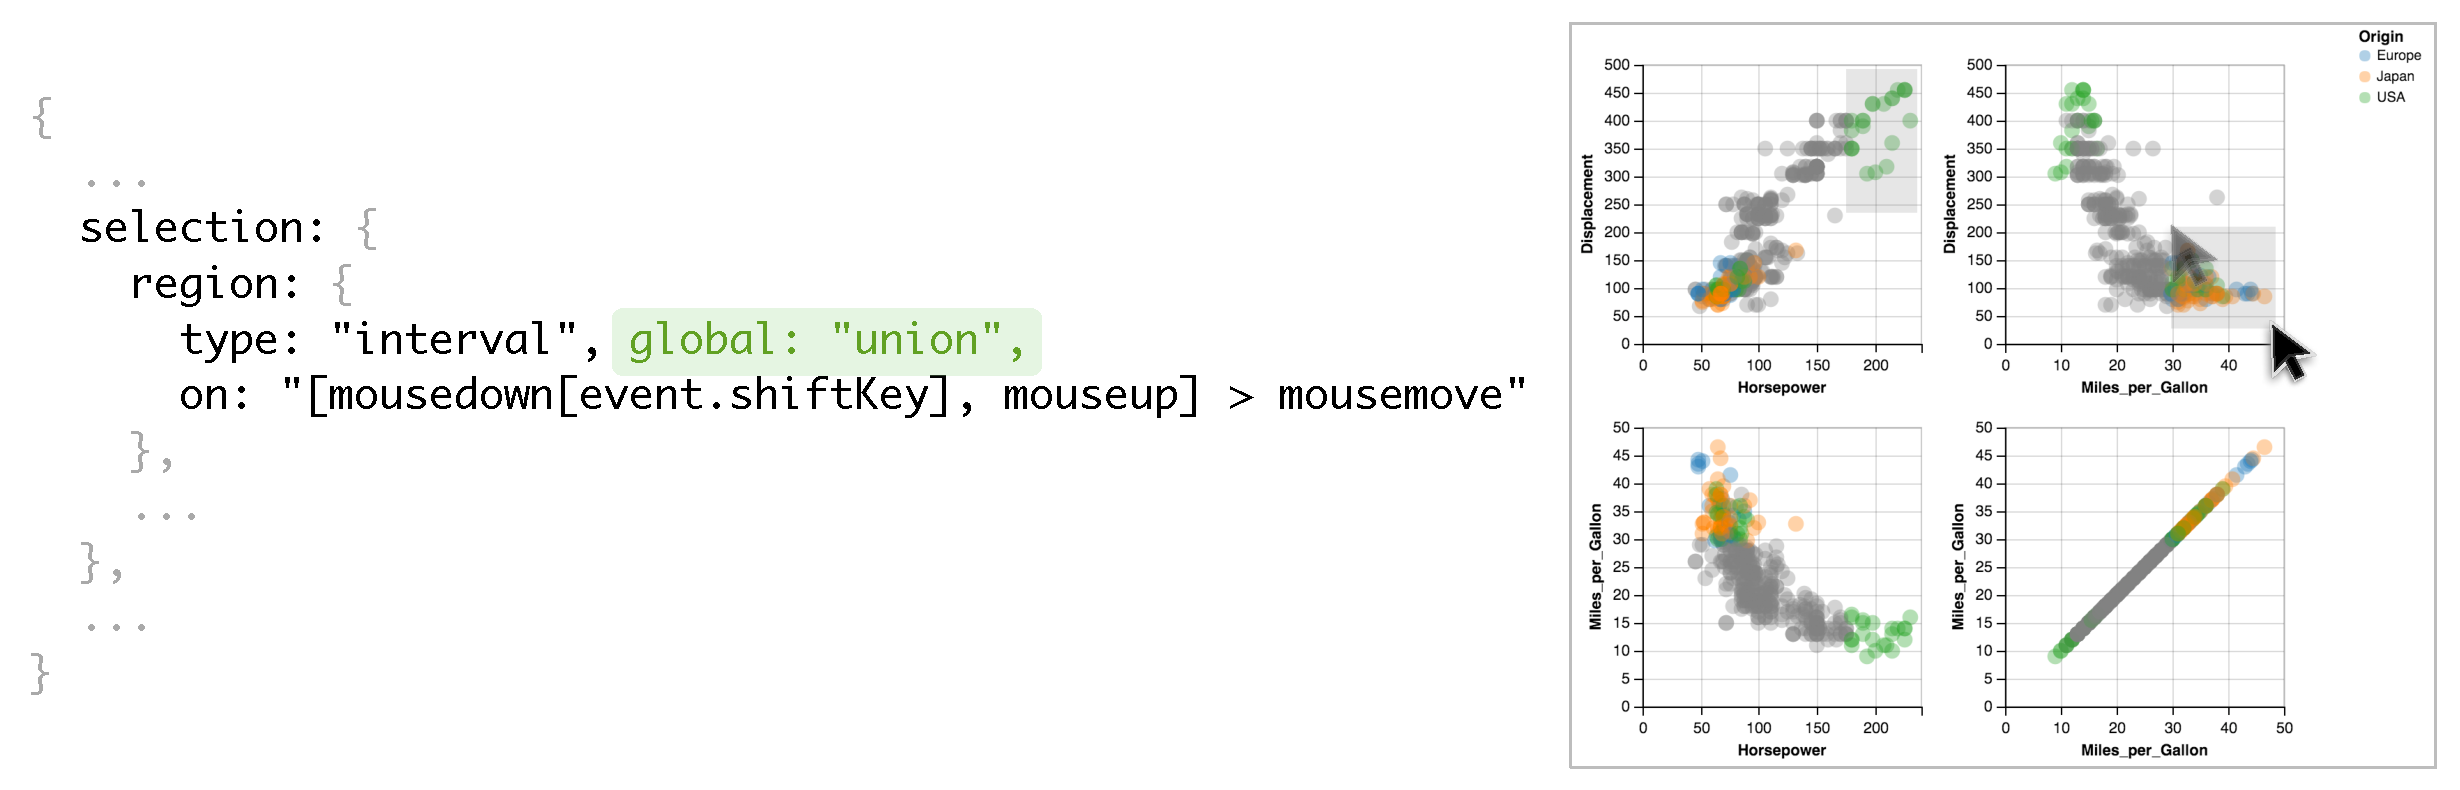
\includegraphics[width=\columnwidth]{resolveUnion}
  \caption{Resolving the \texttt{region} selection to \emph{union}
produces a brush in each cell, and points highlight if they fall within any of
the selections.}
  \label{fig:vl:resolveUnion}
\end{figure}

\begin{figure}[h!]
  \centering
  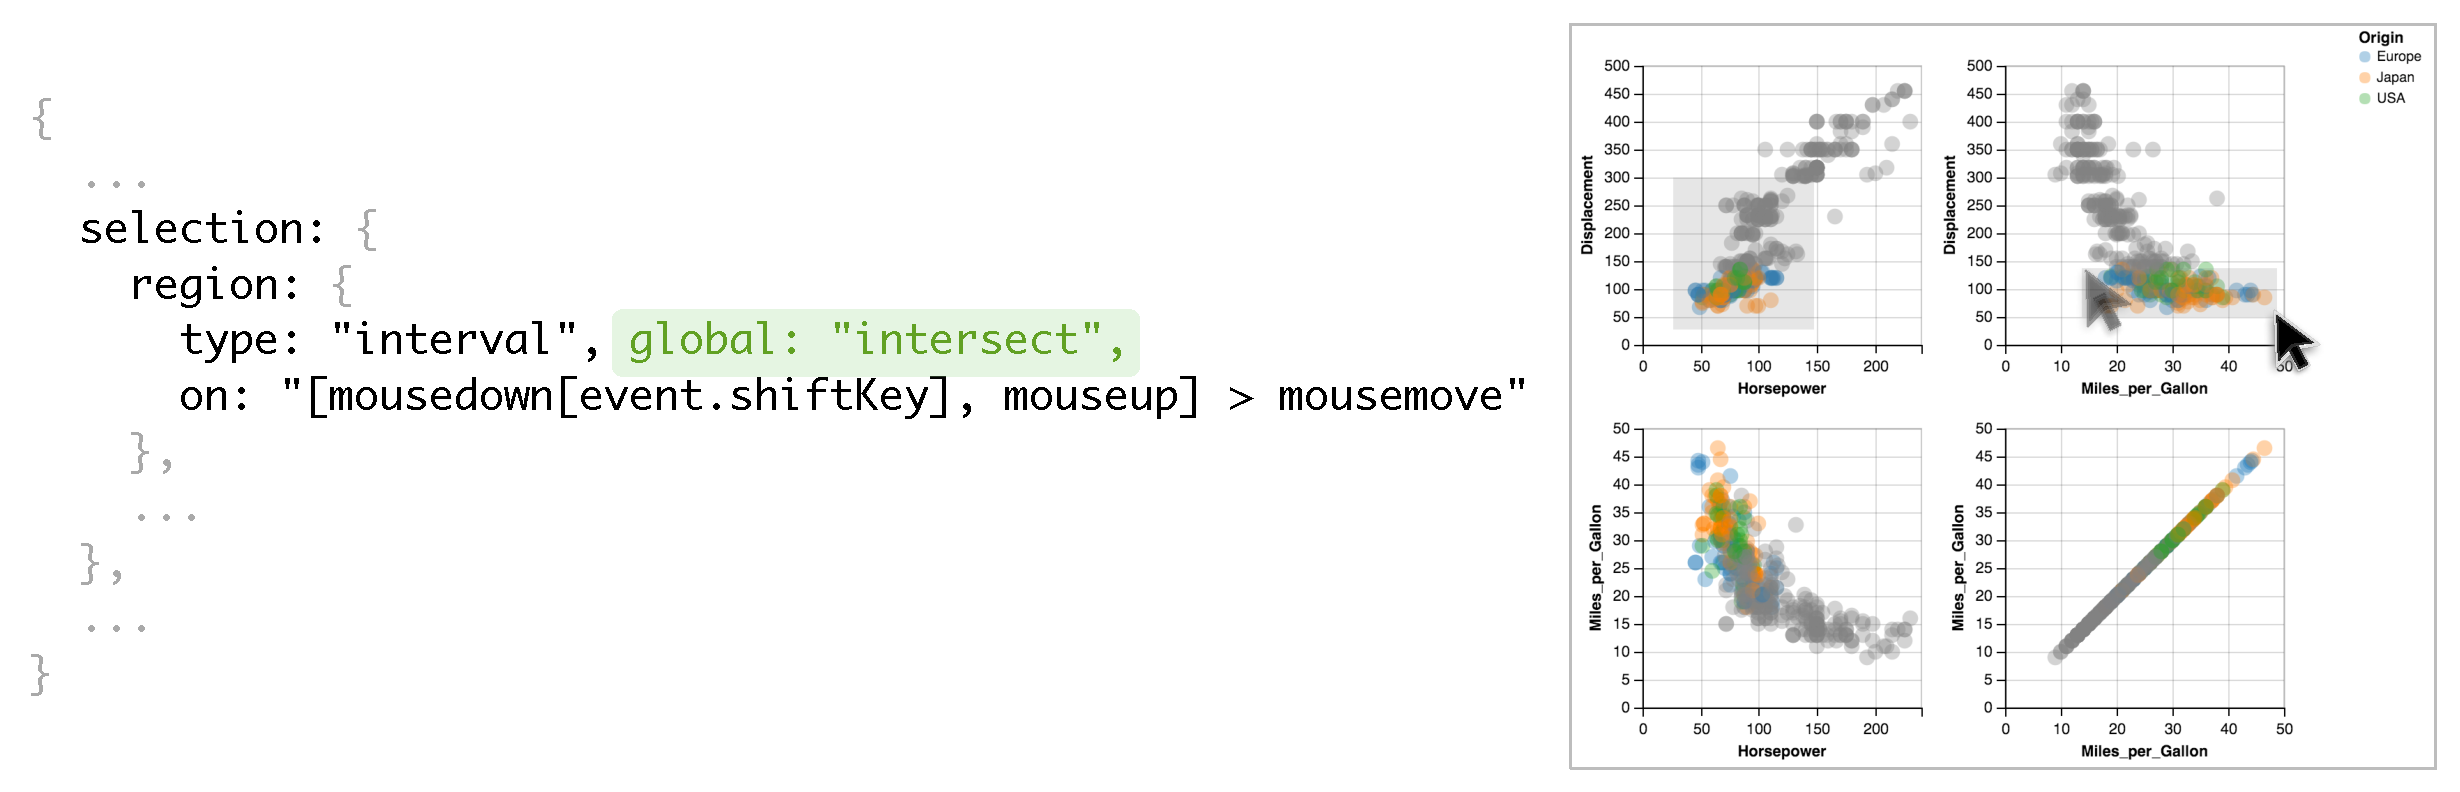
\includegraphics[width=\columnwidth]{resolveIntersect}
  \caption{Resolving the \texttt{region} selection to \emph{intersect}
produces a brush in each cell, and points only highlight if they lie within all
of the selections.}
  \label{fig:vl:resolveIntersect}
\end{figure}